\section{Complete Traceability}
\label{sec:discussion}

Through formal definitions in the previous section we highlight two critical facets -- the semantics and completeness -- in establishing traceability. In our experience, we found that just being able to trace a requirement to a target artifact that satisfies it, say a line of code, is not useful; a holistic view of how that line of code in conjunction with other related lines of code satisfy the requirement provides meaningful information to perform analysis such as assessing the impact of a change. By defining a trace from requirements to the set of target artifacts, we advocate that traceability be captured in a way that upholds its semantic rationale. Further, we also found that many analyses that are performed using sets of trace links without a clear picture whether the trace links are adequate for the purpose.\mike{Which analyses are we talking about here?  This seems like a bold, and unsupported claim.}  By considering $SOS$ trace links and complete traces for each requirement, we can assess analyses related to requirements satisfaction traceability on a proper semantic foundation.  In this section, we elaborate on how the semantic foundations in the previous section help us understand, assess, and use traceability precisely.

%that we explain in the previous section not only provides an in-depth understanding of how the system satisfies requirements but acts as a metric to assess the quality of traceability established for a system and enhances the precision of analysis using the traceability information.

\subsection{Categorizing the Set of Support}

Establishing $ASOS$ for a requirement, one gets a clear picture of the all possible ways that requirement is satisfied. This information helps categorize each target artifact into one of the following groups for that requirement.  The relationships are illustrated graphically in Figure~\ref{fig:maymust}, and explained formally below.
\begin{itemize}
  \item \textbf{MUST} elements - the target artifacts that are present in all the sets of support for a requirement (black triangles in Figure~\ref{fig:maymust}).
      %$$ MUST_x = \{\forall i (S_xi \in \Sigma_x) \mid \bigcap S_xi \}$$
      $$ MUST (r) = \bigcap \ ASOS(r) $$

  \item \textbf{MAY} elements - target artifacts that are used in some, but not all, sets of support (red dots in Figure~\ref{fig:maymust}).
      $$MAY(r) = (\bigcup ASOS (r)) \setminus MUST (r) $$

  \item \textbf{IRRELEVANT} elements - target artifacts that are not in any of the set of support (green stars in Figure~\ref{fig:maymust}). $$IRR(r) = I \setminus (\bigcup ASOS (r))$$
\end{itemize}

\begin{figure}[htb]
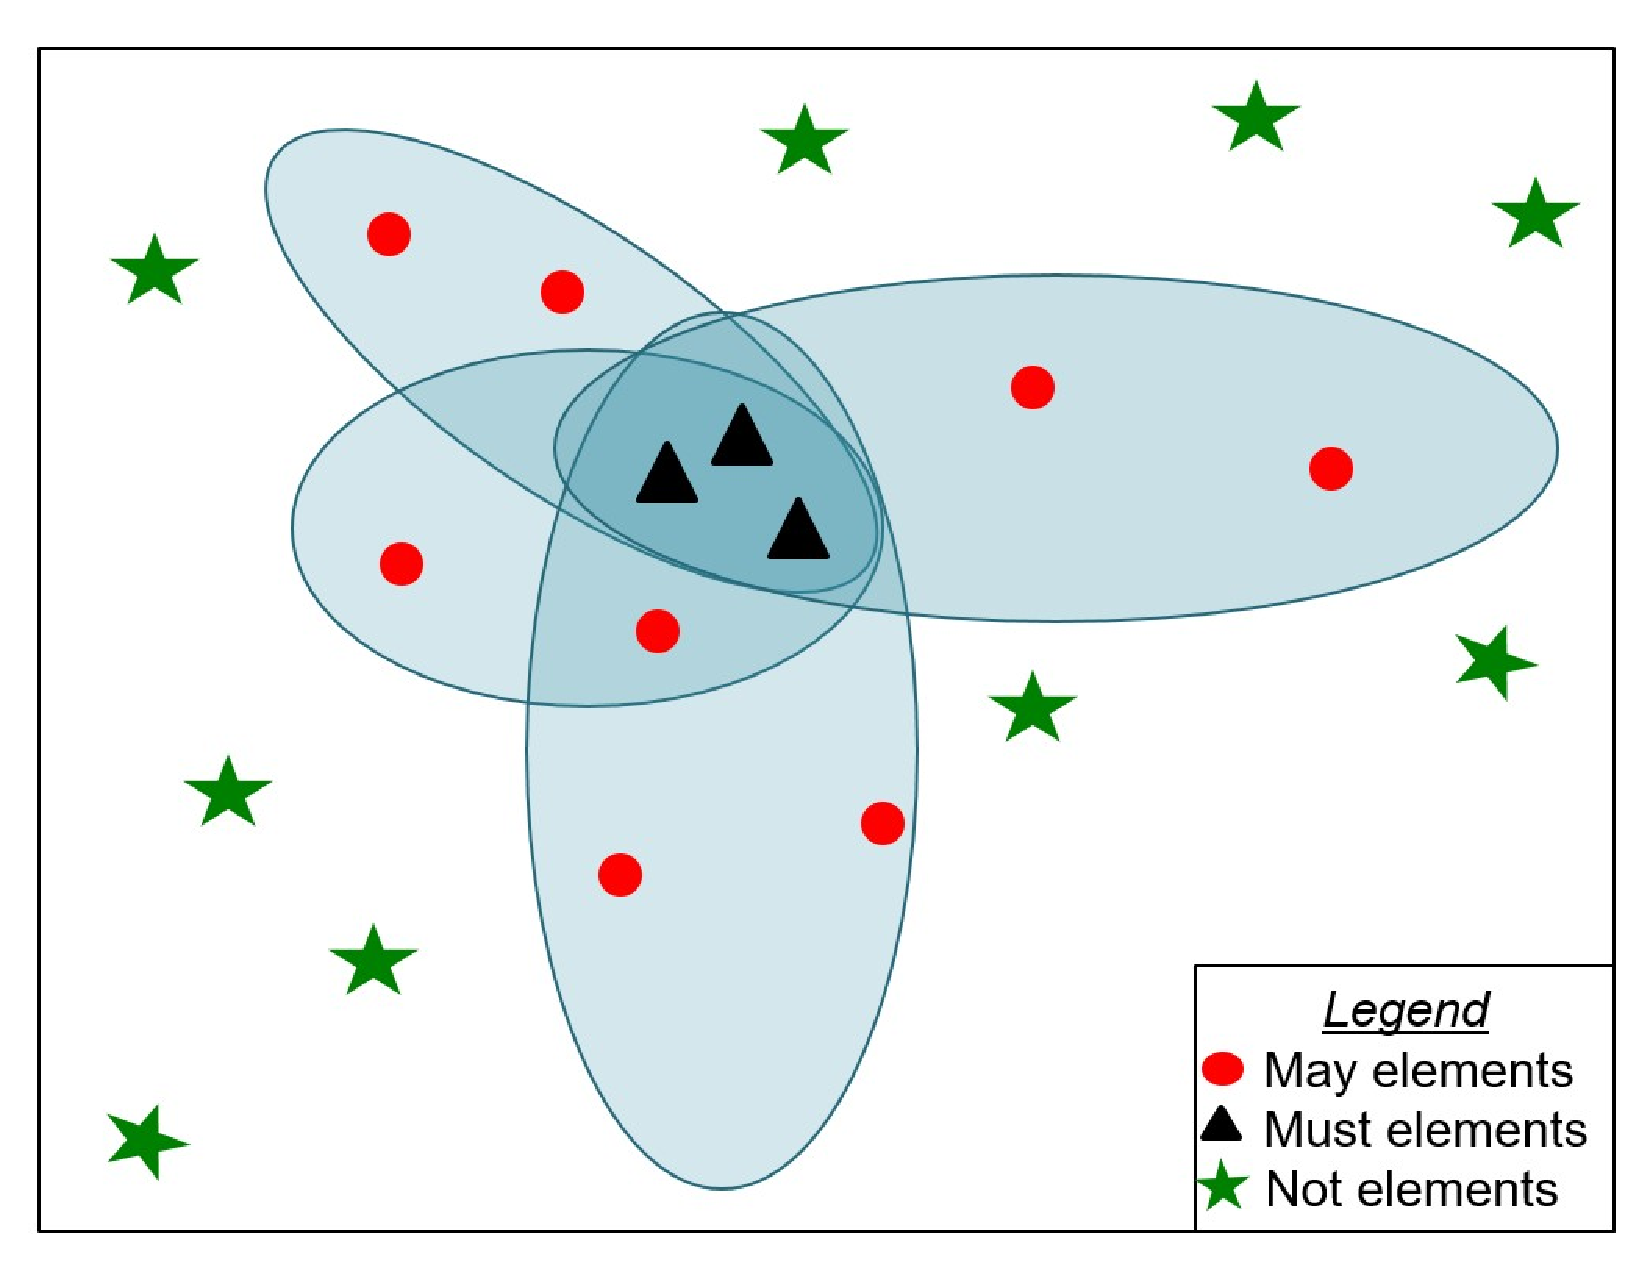
\includegraphics[width=\columnwidth]{images/may_must.pdf}
\caption{May - Must - Irrelevant Set of Support}\label{fig:maymust}
\end{figure}

This categorization helps identify the role and relevance of each target artifact in satisfying a requirement. The MUST elements are those target artifacts that are absolutely necessary for the requirement satisfaction. Hence, any change to these elements will most likely impact on each other. On the other hand, MAY elements indicate those target artifacts that satisfy the requirement in one of the possible ways.  Any change to just one of these elements will not affect the satisfaction of that requirement. The IRRELEVANT elements are never required to satisfy the requirement, so neither does a change in these artifacts affect the satisfaction of the requirement, nor does a change in the requirement necessitate a change in these elements (at least in terms of satisfaction).


\subsection{Using Traces for Precise Analysis}

The categorization of the set of support to be useful in several analyses:

\paragraph{Impact Analysis}: The $ASOS$ set improves understanding of how a change in the requirement will affect the target artifacts and vice versa. While the $ASOS$ as a whole gives a clear picture of various ways a requirement is satisfied by the system, the categorization of target artifacts helps precisely assess and plan when and where the changes have to be implemented. The $MUST$ elements are those target artifacts that are highly likely to change with any change in the requirement, whereas not all $MAY$ elements may need to be changed. On the other hand, if the $MUST$ set is empty ($MUST(r) = \emptyset$) -- there are no common target artifacts between the sets of support -- it indicates that the requirement has been (intentionally or unintentionally) implemented in independent ways, such as fault tolerant systems. For such requirements, one has to carefully analyse and decide if the target artifacts in all or one disjoint set needs to be changed. These analysis could be performed either from the perspective of one or all requirements of the system. 

From the target artifact side, this categorization helps analyse their \anitha{degree of freedom?} to change. Say, we decide to change a target artifact in the $MAY$ set for a requirement. While one might think that it is safe to change this artifact since it does not affect that requirement's satisfaction, an examination of the $ASOS$ sets of other requirements helps identify if it is indeed safe to change that artifact. If it is present in the $MUST$ set for another requirement, then a change to this artifact will definitely impact that requirement. However, if it is in the $MAY$ sets for all the requirements, then it is clearly safe to change. This categorization helps us to precisely assess critical dependencies between the target artifacts and the satisfaction of requirements and thus enables a precise bi-directional impact analysis of a change.

%have to remove any SOS
%take each target artifact and trace to the requirements it satisfies, one can get clear idea about all the requirements it satisfies. If we decide to change a target artifact as long as it is not in any of the MUST sets for any requirement, it becomes evident that it will not affect the satisfaction of any requirement.

\paragraph{Verification and Validation}

Complete traceability can assist in tailoring verification and validation in systems. For instance, if several requirements have a certain target artifact in their $MUST$ set, say an particular assumption, it reveals the importance of focusing V\&V attention on that artifact. Along the same lines, for a system with a complex architecture (components that each have functionality) such as  system of systems, this categorization helps identify components that is critical to satisfy most requirements. This helps plan verification strategies.

If we examine changing a target artifact that appears $MUST$ set for any requirement, then this requirement must be re-verified. However, if it appears in the $MAY$ set for the requirement, then we can instead remove any sets-of-support that contain the element; as long as there still exists at least one set of support for the requirement, no reverification is necessary for that requirement. 

Further, the notion of complete traces helps to assess if requirements are satisfied by the system in an unintended manner. It is well known that issues such as vacuity~\cite{Kupferman03:Vacuity} can cause requirements to be satisfied in a trivial manner. Even for non-vacuous requirements, it can be the case that requirements can be satisfied using a much smaller portion of the system than intended because they are incorrectly specified.  By capturing all the set of support and categorizing them, it is possible to examine whether the MUST set corresponds to expectations on the system, or, if more rigor is required, to examine each set of support individually to see whether it matches expectations.
%one could evaluate if there are unintended target artifacts that might cause the requirements to be satisfied. %In one of our experiments using an infusion pump system software, while capturing the $RST_m$ for a requirement we discovered that there was a requirement whose set of support included a not the one that  to be trivially satisfied. When we

\paragraph{Completeness Checking}

By getting all the sets of support for all requirements of the system and categorizing them, one can get a clear picture about the role of target artifacts in satisfying the requirement(s). By reversing the direction of the complete requirement satisfaction trace, one can find if there are target artifacts that do not trace to any requirement.  This can be performed by examining the minimal set of target elements used by {\em any} SOS for {\em all} requirements, in other words the \{$\bigcap IRR$\} set of all requirements.  If so, it is a possible indication of ``gold plating" or missing requirements. In other words, it helps assess if there requirements of the system are completely specified with respect to describing all the behaviors of the system. Being able to assess the coverage of requirements over the model is crucial in the safety critical system domain.
 
\paragraph{Comparing Traceability Approaches}
%\anitha{I am not happy with this now.... But I do want to say something along these lines... }
%\mike{I agree, but I have not made any changes to the section.}
There is substantial interest within the Requirements Engineering research community (and our immediate research group) towards automating the construction and maintenance of traceability links.  To that end, there are repositories such as \mike{Name of Jane's repository HERE + citation} containing many example systems, each with a reasonably complete set of requirements and target artifacts and with trace links constructed by groups of experts.  It is then possible to benchmark automated and semi-automated traceability approaches against vetted sets of trace links.

We are, in general, very supportive of this approach: benchmarking against a reasonable set of candidate models has been very important in several areas of computer science research, including CPU, GPU, and compiler performance~\mike{citations here}, performance of SAT/SMT solvers and model checkers~\mike{cite SATcomp and SMTcomp}, and many other areas.  However, it can also be misleading if the benchmark problems are not carefully selected or if results are incorrectly computed, as described in, e.g., several articles critical of benchmarking for CPU/GPU performance~\mike{citations here}.

For traceability research, the usual standard measures for examining the performance of different approaches is in terms of {\em precision} and {\em recall} against the ``gold standard'' set of traceability links that exist in repositories.  Our concern is that, for requirements satisfaction traceability, there are often many such sets of valid links, as we have explored in this paper, so these metrics may be misleading.  One can envision situations in which the gold standard pursues one set of support and the automated approach pursues another, leading to low precision and recall scores.  A close examination of traceability links and categorizations such as the ones we have explored may be useful to provide more accurate measurements of the quality of automated approaches.  If requirements have more than one SOS, the gold standard should probably contain each of these arguments.  In addition, the ability to characterize trace links as $MAY$ or $MUST$ may be a fruitful direction of future research for automated approaches to constructing trace links.


%To the best of our knowledge, the existing benchmarks and ways to establish benchmarks to assess the effectiveness of traceability techniques or evaluate the trace links is not guaranteed to be flawless. The correctness and thoroughness of the benchmarks are in someway assumed and not rigorously assessed. A number of research work compute the precision and recall of their traceability approaches by using such benchmarks. We believe that to evaluate the completeness and precision of those benchmarks we need to first rigorously characterize it. The requirements satisfaction trace defined in the previous section helps us move forward in that direction. Since the trace is based on establishing a satisfaction argument it is straightforward to verify/validate the precision of each trace (which is 100$\%$). The complete requirements satisfaction trace, as the name suggests, is defined to capture traces to all sets of support. While this may sound theoretical, once established it will be the perfect benchmark to compare results to.

\mike{Stopped here.  Not sure we want the discussion below at all.}
Contrary to the general notion that it is impossible or extraordinarily difficult to identify all trace link in practice~\cite{stravsunskas2002traceability}, some of the initial results from our recent efforts~\cite{IVCTechReport} indicate that such complete requirements satisfaction trace can be established, in fact automatically in the realm of formal methods and model based developments. In the next section, we breifely describe our prior work and our plans to extend it to establish complete traceability. While the details the approach and initial results are not in scope of this paper, an interested reader is directed to~\cite{IVCTechReport}.



%
%
%
%\newcommand{\bfalg}{IVC\_BF}
%\newcommand{\ucalg}{IVC\_UC}
%\newcommand{\ucbfalg}{IVC\_UCBF}
%
%The approach from the previous section establishes trace links between properties at different levels of the system architecture based on inductive validity cores derived from inductive proofs.  For functional requirements, this approach automates the traceability information necessary to establish {\em satisfaction arguments} in the style of \mike{Ref to Will it Work HERE}.  In so doing, it allows a substantial change in how traceability is performed, and to some extent, what traceability {\em means}.  As we explained in the motivating example, there is often more than one way that the requirements could be satisfied by the model, that is, there is more than one set of support for the requirement.  This requires an examination of how we perceive traceability in terms of which model elements (equivalently: subcomponent properties) are {\em always required} by any proof, which elements are {\em sometimes required}, and which elements are never required, which we call {\em must} and {\em may} trace links.  It also brings up fruitful discussions on how architectures are constructed and the nature of the links between requirements and architecture.
%
%\subsection{Overhead of Computing IVCs and Minimality of Generated IVCss}
%In our accompanying technical report~\cite{}, we present two algorithms that are used to compute IVCs and an experiment to examine the quality of the approach.  Our primary concerns are the {\em efficiency} and {\em
%minimality} of the approach.  Efficiency is computed in terms of wall-clock time: how much overhead does the IVC algorithm introduce?  Minimality is determined by the size of the IVC: cores with a smaller number of
%variables are preferred to cores with a larger number of variables.  Both of the proposed algorithms are {\em sound}, in the sense that from the IVC, it is always possible to reconstruct the proof, so they do not miss trace links.
%
%In~\cite{}, we present two algorithms that pose different tradeoffs between these goals.  The first algorithm, called \ucalg, uses UNSAT cores to determine an IVC and runs very efficiently (on average, for the 477 models in the experiment, about 15\% overhead over performing the proof when using the z3~\cite{} solver), but is not guaranteed to yield a minimal IVC; on average, it yields a core that is 21\% larger than minimal.  The second algorithm, called \ucbfalg, adds a ``brute force'' postprocessing stage that guarantees that the generated core is minimal, but adds, on average, a greater than 30-times slowdown to the proof.
%
%\subsection{On-Demand Traceability}
%
%Because the efficient algorithm (\ucalg) adds very little overhead to the model-checking process, which is itself quite efficient, we can think of it as providing ``on-demand'' traceability.  In most traceability approaches, maintenance of trace links is a very significant concern and one of the reasons that finding and fixing errors is so expensive in critical systems.  However, with our approach, it is straightforward to provide users with accurate trace information consistent with the model immediately after changes are made.  This allows traceability to easily be used as an {\em exploratory} analysis early during requirements gathering and architectural prototyping.  We have used it in this way in the DARPA SOSITE project, where we used traceability information to check whether we were writing appropriate requirements and to check ``semantic vacuity'', as will be described in a following section.
%
%In hand-generated trace links for satisfaction, there is a potential for both missing required traceability links and addition unnecessary traceability links.  In our approach, there is an interesting tradeoff in terms of usability of trace links: is it more important that they are inexpensive to generate or that they are minimal?  In our approach, for functional requirements, if we overapproximate the set of required model elements, does this still provide value?  Our claim of (on average) 21\% larger sets of support is perhaps misleading: for the GPCA models, which contain hundreds of possible subcomponent requirements that contribute to a proof, the \ucalg\ set of support is either the same as the \ucbfalg, or it has between 1 and 5 extra elements (e.g., 10 elements vs. 8 elements).  For users seeking to understand the relationships between system and subcomponent requirements, it seems that the faster algorithm may yield reasonable results.  On the other hand, if we want to use the tool for some kind of certification-related activity, it is likely worth the extra cost to get more exact results.
%
%\mike{more here???}

%\subsection{Categorizing Trace Links}
%We often describe ``the'' traceability matrix for a system, tracing requirements to lower-level requirements, design artifacts, or implementations.  However, at least for functional requirements, it is more correct to speak of ``a'' traceability matrix, because there are multiple minimal sets of model elements that lead to a proof.
%
%
%For instance, in safety critical system domain for fault tolerance one could intentionally add multiple ways to satisfy a requirement, or one could unintentionally add model functionality that leads to multiple ways of satisfying a requirement. By iteratively using our approach to query the solver for different sets of support until it does not find any, we can obtain all the sets of support for a requirement. Getting all the sets of support is nothing but establishing complete traceability between the requirements and all the parts of the model that contribute to satisfying it.
%
%%\subsection{Categorizing Support Elements}
%
%Establishing complete traceability paves way to indepth understanding of the model. Given all sets of support for a requirement, one could categorize them into the following, as illustrated in Figure~\ref{fig:maymust}:
%\begin{itemize}
%  \item MUST elements - support elements that are present in all the sets of support
%  \item MAY elements -  elements in set of support, but not common to all the sets of support
%  \item IRRELEVANT elements -  support elements of the model that are not in any of the set of support
%\end{itemize}
%
%\begin{figure}[htb]
%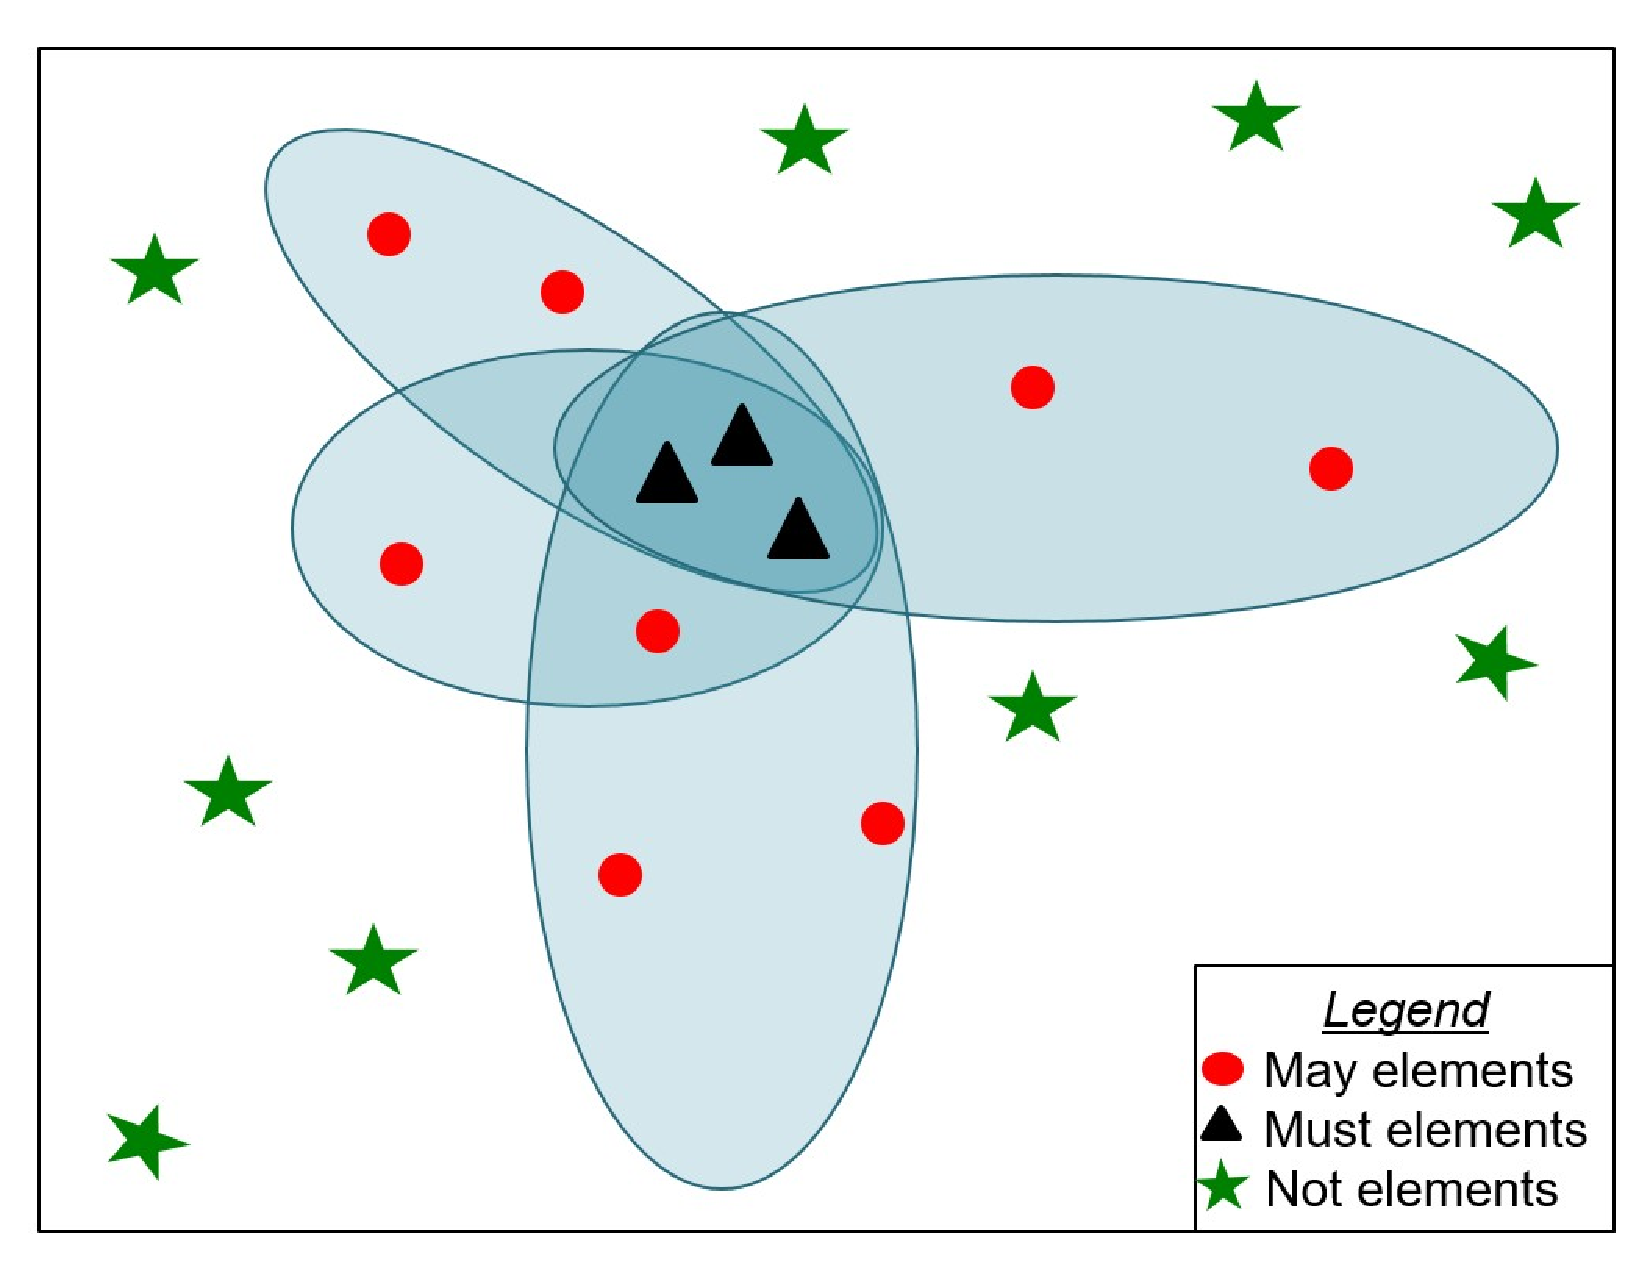
\includegraphics[width=\columnwidth]{images/may_must.pdf}
%\caption{May - Must - Irrelevant Set of Support}\label{fig:maymust}
%\end{figure}
%
%The MUST elements indicate that those parts of the model are absolutely necessary for the requirement to be satisfied. Hence, any change to either requirements or one of these elements will have an impact on the other. On the other hand, MAY elements indicate the parts of the model that satisfy the requirement in one of the possible ways. Any change to just one of these elements will not affect the satisfaction of the requirements. The NOT elements are in no way related to satisfying the requirements. When performing impact analysis of a change in requirements or dependency analysis to assess the effect of changing the model, this traceability provides a complete picture of all the dependencies.
%
%
%



%
%
%\subsection{Traceability Coverage}
%
%While establishing complete traceability is useful, to the best of our knowledge, how elaborately should traceability be captured is not well discussed in the literature. The question is "Should traceability be quantified?" The usual trace relationships between the system (or its model) and the requirements is "satisfies" or "implements" etc. We recommend that the relationship explicitly state whether traceability captures "one way to satisfy/implement" or "all the ways to satisfy/implement" the requirements. Making it explicit helps precisely realize the benefits of traceability.
%
%\anitha{in progress.}....

